\documentclass[conference]{IEEEtran}
\usepackage[english]{babel}
\usepackage{multicol}
\usepackage{multirow}
\usepackage{url,hyperref,graphicx,float,times}
%\usepackage{sectsty}
%\usepackage{authblk}
\usepackage{textcomp}
\usepackage{cite}
% \graphicspath{{../pdf/}{../jpeg/}}
% \DeclareGraphicsExtensions{.pdf,.jpeg,.png}
\usepackage[caption=false,font=footnotesize]{subfig}

\usepackage{url}

\begin{document}

\title{Title}

\author{\IEEEauthorblockN{Ching-Chun (Jim) Huang} \IEEEauthorblockA{Department of\\Computer Science and Information
Engineering\\National Cheng Kung University, Taiwan\\ No.1, University Road, Tainan City 701, Taiwan (R.O.C.)\\ Email:
jserv@ccns.ncku.edu.tw} \and \IEEEauthorblockN{Chung-Fan Yang} \IEEEauthorblockA{Department of Electrical Engineering\\
National Cheng Kung University, Taiwan\\ No.1, University Road, Tainan City 701, Taiwan (R.O.C.)\\ Email:
E24026048@mail.ncku.edu.tw}}

\maketitle

\begin{abstract}
\end{abstract}

\section{Introduction}

\section{Related Work}

\section{Methodology}

    Based on the works presented above, we have methods to measure the overall wake-up latency and context-switch
    latency, using cyclictest and lmbench. Also, it's able to show that the CFS algorithm has O(1) complexity on
    selecting next task, giving static latency. Thus, overall  and parts of latency of a Linux system can be determined,
    but the measurement methodology and tool of scheduler latency, shown in figure \ref{fig:latency_timeline}, are
    lacking. Therefore, we developed a evaluation tool of scheduler duration jitter, based on methodology method of A
    Decade of Wasted Cores \cite{Lozi:2016:LSD:2901318.2901326}. This methodology method enabled us to record the
    scheduler states including, executing process ID (PID), PID in scheduler run-queue, context switch points, timer
    interrupt execution, scheduling events, etc. on per processor core basis. This methodology method differs from
    profiling based methodology tools, e.g. perf \cite{perf}, lacking high fidelity, all-recorded profiling result of
    the target system. Our proposed tool can do full-detailed record in microsecond scale on x86-64 and ARM system,
    which is able to capture the impact to real-time performance of occasional short-burst scheduler events, which only
    last less that 10us. These events are mostly not shown in the result of sampling based measurement which focus on
    average-case execution time(ACET). By analyzing full-detailed record, we are able to not only capture the worst-case
    execution time (WCET), but also understand the cause of these incidents.

    In addition, the behavior and loading characteristic of typical work-load used during test in above works, e.g.
    hackbench, stress \cite{rt-tests}, etc. are far from the real-world real-time applications. These problems not only
    would reduce the significant of target system jitter measurement, but also will make incidents, harming the
    real-time performance, obscure. In result of this frustration, we also created a testing framework hosing an
    algorithm which resembled a real-time robot control system execution behavior, named mctest. This work-load
    application has the ability to be compiled either as user-space program or kernel module, provides observation of
    the characteristic of target application execution in both user-space and kernel-space. This would gives the insight
    of system-call and user-space I/O overhead, which does not exist in kernel module. In addition, mctest would do a
    series of identically executions and record the execution time of each turn. These records can be used to determined
    the execution jitter of the application on the real-time system, which besides wakeup latency. This could be used to
    reflect to the system-call overhead of the system. We have been utilizing mctest as the testing work-load and jitter
    measurement tool during methodology.

    \begin{figure} \centering 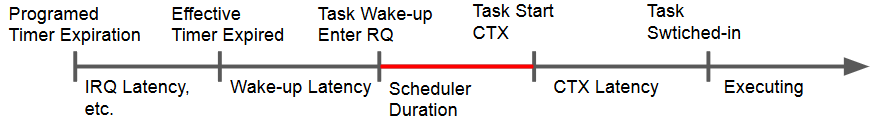
\includegraphics[width=3.5in]{img/latency_timeline.png} \caption{Task Wake-up Latency}
    \label{fig:latency_timeline} \end{figure}

\section{Experiment}

    In aid of these developed tools and work presented above, we did multiple experiments and measurement of 2 ARM
    Cortex-A9 based platform, shown in table I. These platforms are selected as CMP based ARM system are emerging and
    being used in a wide field of applications. These systems are running buildroot \cite{buildroot} built Linux with
    kernel version 4.4 and PR\textunderscore RT \cite{preemptrt} patches.

    \begin{table*}[] \centering \caption{Experiment Platforms} \begin{tabular}{|l|c|c|} \hline Platform Name & Altera
        SoC FPGA Development Kit & Freescale i.mx6 Sabre \\ \hline Processor & 2x ARM Cortex-A9 & 4x ARM Cortex-A9 \\
        \hline Memory & 1 GB & 1 GB \\ \hline Additional configuration & None & \begin{tabular}[c]{@{}c@{}}L2 Cache
        locked down to CPU1,\\ Isolated CPU1,\\ Enabled tickless on CPU1 \\ Real-time task pinned to CPU1 \end{tabular}
    \\ \hline \end{tabular} \end{table*}

    Our experiment begins with known tuning practices which includes processor isolation \cite{isolatedcpu}, tickless
    feature of kernel \cite{tickless}, L2 cache lockdown. We compared the measurement result of mctest with and without
    these tuning techniques on Freesacle i.mx6 Sabre platform. Measurement results are shown in figure
    \ref{fig:imx6_mctest_v}, \ref{fig:imx6_mctest_iso}, and \ref{fig:imx6_mctest_lock}, verifying the effectiveness of
    these known tuning techniques and providing results as a baseline. We are able to see the WECT with and without
    tuning are 100us and 100us. This gives us the hint that the scheduling would harms the real-time performance. This
    scheduling overhead could be separated into 2 parts, scheduler overhead and cache contention on SMP system. With L2
    Cache lockdown technique we are able to mitigate most of the cache contention, but still resulting some degree of
    jitter about 100us

    \begin{figure} \centering 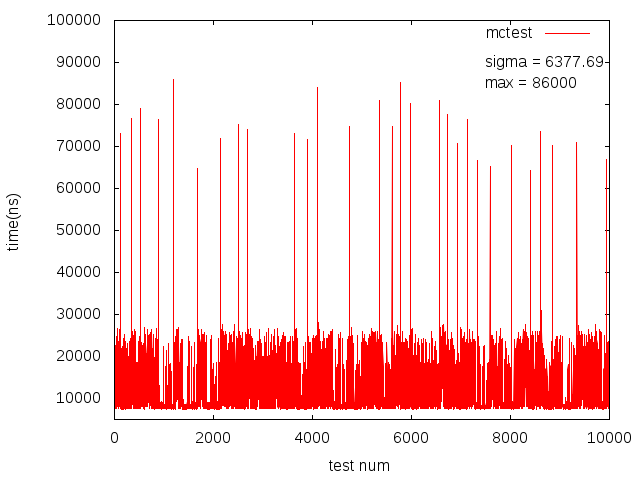
\includegraphics[width=3in]{img/mctest-none.png} \caption{Mctest on i.mx6 Sabre}
    \label{fig:imx6_mctest_v} \end{figure}
    
    \begin{figure} \centering 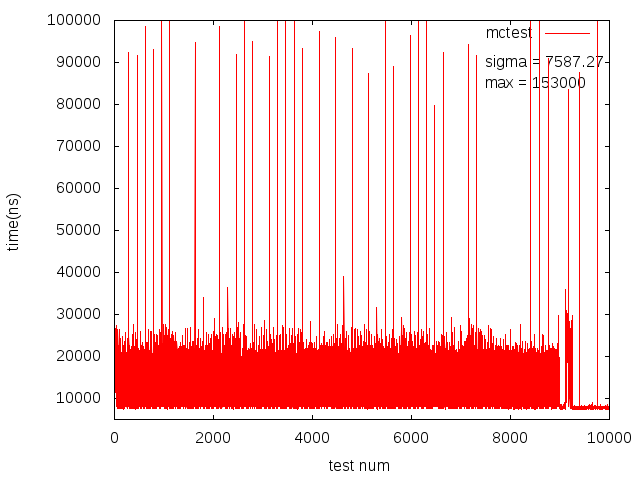
\includegraphics[width=3in]{img/mctest-iso.png} \caption{Mctest on i.mx6 Sabre with
    isolated cpu and tickless feature} \label{fig:imx6_mctest_iso} \end{figure}
    
    \begin{figure} \centering 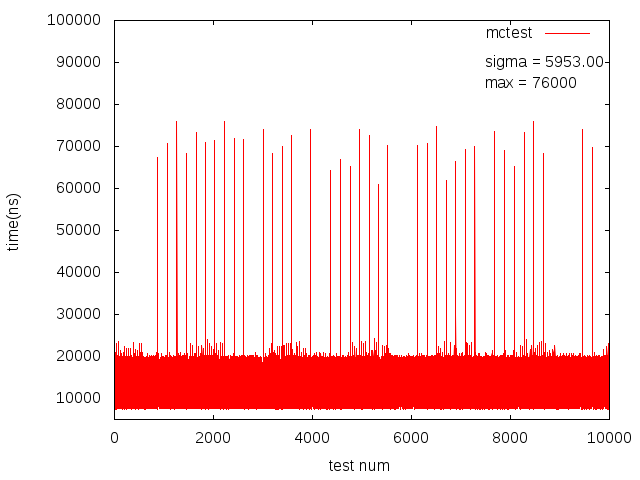
\includegraphics[width=3in]{img/mctest-lock.png} \caption{Mctest on i.mx6 Sabre with
    isolated cpu, tickless feature and L2 cached lockdown} \label{fig:imx6_mctest_lock} \end{figure}
    
\subsection{System Call Overhead and Kernel Mode Linux}

    In addition, we compared the user-space mctest result with kernel space measurement, shown in figure
    \ref{fig:imx6_mctest_k_v} and \ref{fig:imx6_mctest_k_lock} with WECT of 50us and 50us. With these result, we are
    able to identify the sources of jitter are system calls. To mitigate these, we first proposed to rewrite real-time
    applications as kernel modules. But this is tedious and making the debugging process difficult. Thus, we proposed a
    second approach, Kernel Mode Linux(KML) \cite{KML} \cite{KMLConf}. KML enables the ability for specified user-space
    program running in kernel memory space. Thus, system calls become jump instructions, not instruction trapping the
    processor. Also, this would mitigate the cache contention while switching in and out the kernel during system call.
    In addition, we have also rewired system calls, which have vDSO implementations \cite{vDSO}, to use vDSO
    implementation via KML. The result of user-space program running in KML is shown in figure \ref{fig:imx6_mctest_kml}
    with WECT of 20us, which proving the effectiveness of jitter mitigation from KML.

    \begin{figure} \centering 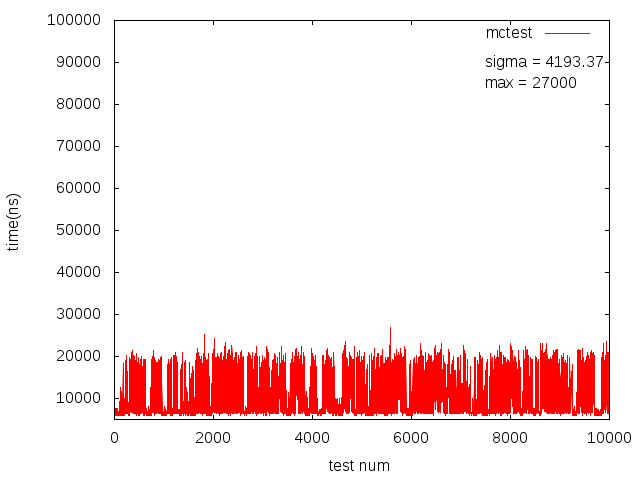
\includegraphics[width=3in]{img/mctest-k-none.png} \caption{Kernel mctest on i.mx6 Sabre}
    \label{fig:imx6_mctest_k_v} \end{figure}
    
    \begin{figure} \centering 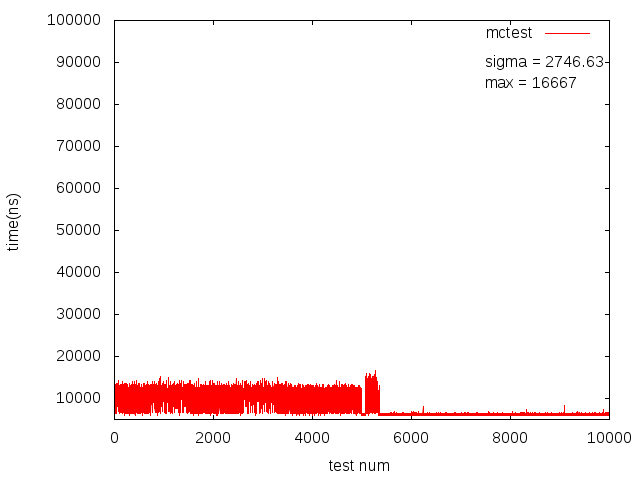
\includegraphics[width=3in]{img/mctest-k-lock.png} \caption{Kernel mctest on i.mx6 Sabre
    with isolated cpu, tickless feature and L2 cached lockdown} \label{fig:imx6_mctest_k_lock} \end{figure}
    
    \begin{figure} \centering 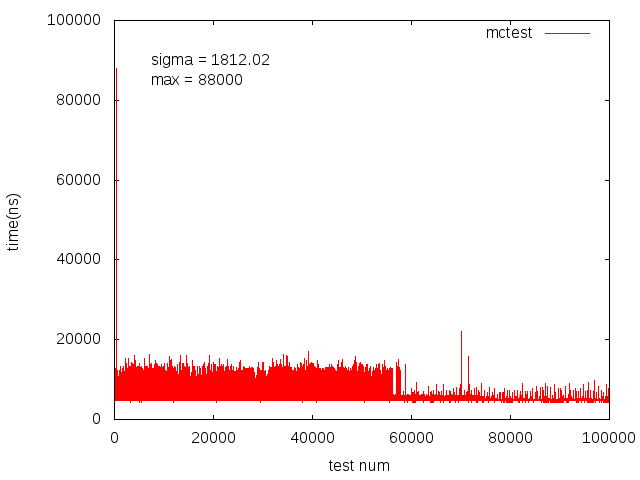
\includegraphics[width=3in]{img/mctest-kml.png} \caption{Mctest on i.mx6 Sabre with
    isolated cpu, tickless feature in KML} \label{fig:imx6_mctest_kml} \end{figure}
    
\subsection{Scheduler Overhead Measurement}
    
    Identifying that scheduler is also a source of jitter, we applied our proposed scheduler profiling tool to evaluate
    and identify of which part of the scheduling process is the source of jitter. Knowing the IRQ latency, and
    context-switching latency, we would like to evaluate the scheduler duration. Traditionally, the latency of this part
    is considered static with the CFS algorithm complexity, designed to be O(1), but real measurement result are
    lacking. Thus, we set our proposed profiler to record the increment of scheduler run-queue and scheduler
    context-switching events with switched-to PID of each processors. A analyzer will process the recorded data and
    gives out the scheduler duration of a specified process, enabling us the understand the scheduling of real-time task
    in SMP system. The result of running a solo instance of cyclictest on SoC FPGA Development Kit is shown in figure
    \ref{fig:sd_solo}. The latency could be considered static with maximum 10us. This result matches traditional
    considerations, but with the interference from other work-load, the jitter will start to emerge.

    \begin{figure} \centering 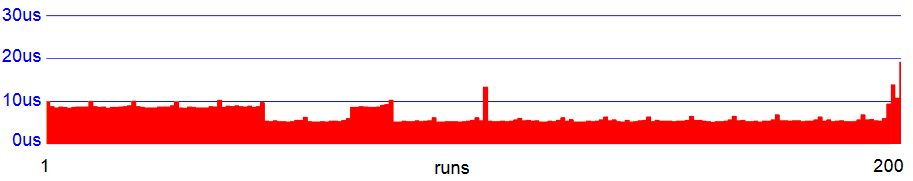
\includegraphics[width=3.5in]{img/sd-solo.png} \caption{Scheduler duration of solo
    cyclictest, no load} \label{fig:sd_solo} \end{figure}

\subsubsection{Overloaded System}

    We created additional work-load, executing alone with cyclictest during profiling session. We created a mild loading
    condition, which has 3 stress threads, and a heavy loading condition, which has 8 stress threads. The result of mild
    loading condition is shown in figure \label{fig:sd_mild}. This result also exhibits a mostly static scheduler
    duration with seldom jitter with maximum of 20us. But putting the system in to heavy loading condition, the result,
    shown in figure \ref{fig:sd_heavy} exhibits random jitter from 10us to 30us. The spread of distribution of scheduler
    duration, shown in figure \ref{fig:sd_heavy_d}, would become wilder. This informs us that the scheduler duration is
    not a static value and will increase alone with the system's load. Also informs that the scheduler duration contains
    but not only contains CFS algorithm task selection process which is proved to be O(1).

    \begin{figure} \centering 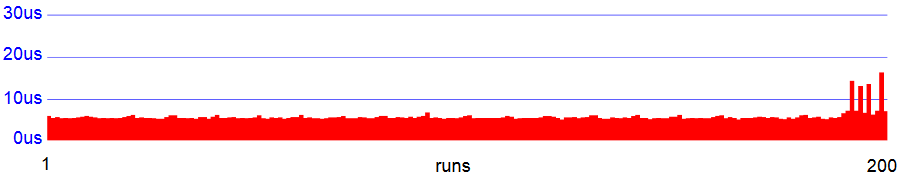
\includegraphics[width=3.5in]{img/sd-mild.png} \caption{Scheduler duration of cyclictest
    with mild load} \label{fig:sd_mild} \end{figure}

    \begin{figure} \centering 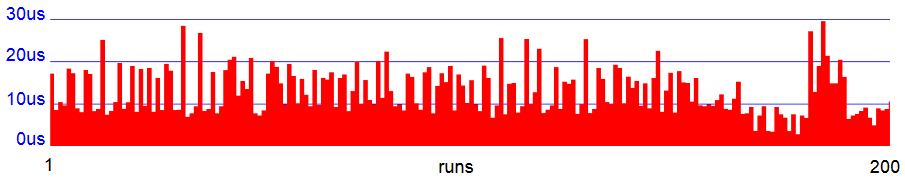
\includegraphics[width=3.5in]{img/sd-heavy.png} \caption{Scheduler duration of cyclictest
    with heavy load} \label{fig:sd_heavy} \end{figure}

    \begin{figure} \centering 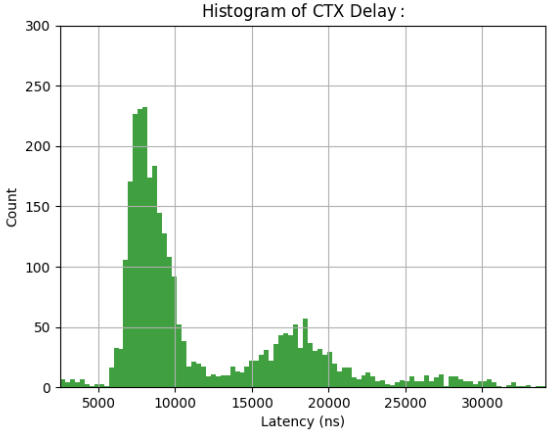
\includegraphics[width=3.5in]{img/sd-heavy-d.png} \caption{Scheduler duration distribution
    of cyclictest with heavy load} \label{fig:sd_heavy_d} \end{figure}

\subsubsection{Short Inter-Arrival Time}

    We also captured large jitter of scheduler duration on a mild loaded system. The experiment is running mctest with
    cyclictest. We pinned kernel module mctest to use first processor, causing cyclictest real-time thread and main
    thread being scheduler onto second processor. On most of the time, this execution schema results the same result as
    cyclictest executing solely in the system. But on some occasions, the cyclictest main thread would be waken-up and
    enter run-queue with short inter-arrival time against the cyclictest real-time thread, which was also being
    waken-up. When this event happened, the scheduler duration will raise to 30us. This result, shown in figure
    \ref{fig:sd_mctest} hints us that not only long term overload system would exhibit large scheduler duration, but
    also short burst a overloading condition during the real-time task scheduling and execution would cause the
    scheduler duration to raise.

    \begin{figure} \centering 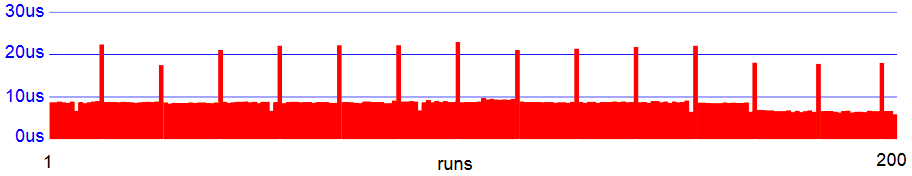
\includegraphics[width=3.5in]{img/sd-mctest.png} \caption{Scheduler duration of cyclictest
    with short inter-arrival time to run-queue against other task} \label{fig:sd_mctest} \end{figure}

\section{Conclusion}

    We have evaluated the real-time behavior of Linux by profiling kernel scheduler and measuring the latency of various
    kernel variants. An intensive interrupt load can cause long OS latencies due to the design of the interrupt
    processing mechanism. We proposed new tools to visualize task scheduling in fine-grained scale(microsecond level).
    This enabled us not only focusing on interrupt latency, but also scheduler durations, lock, and etc. It would thus
    be highly desirable to combine existing techniques, e.g KML, isolated CPU, tickless kernel, to improve task
    responsiveness under various target application characteristics, on top of PREEMPT\textunderscore RT.

\bibliographystyle{IEEEtran}
\bibliography{references}

\end{document}
